\documentclass[resume]{subfiles}


\begin{document}
\section{Acquisition et synchronisation}
Il faut prendre en compte :
\begin{itemize}
\item Délais de propagation
\item Effet doppler (émetteur / récepteur mobile)
\item Fading
\item Variations locales des oscillateurs (température, variations, etc...)
\end{itemize}
La fréquence est connue à peu près, la phase est inconnue. Les outils suivants permettent de palier à ces problèmes (en partie) :
\paragraph{Amplifier Gain Control AGC} : Correction de l'amplitude sur l'amplificateur. Constitué d'un LNA (Low Noise Amplifier), d'un ADC et un multiplicateur digitals
\begin{center}
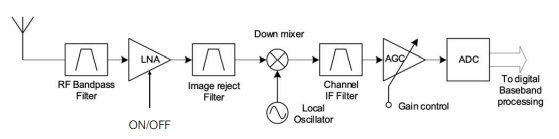
\includegraphics[width=\columnwidth]{img_1.png}
\end{center}
\paragraph{PLL / FLL} : Frequency locked loop / phase locked loop
\paragraph{Voltage Controlled Oscillator VCXO} $f(t)=f_0+K_0v_{in}(t)$
\subsection{Récupération de la porteuse}
Réponse de la forme
$$H(s)=\frac{K\frac{G(s)}{s}}{1+K\frac{G(s)}{s}}\qquad G(s)=\frac{1+\tau_2 s}{1+\tau_1 s}$$
\subsection{Récupération des symboles}
Utilisation de :
\begin{itemize}
\item Beacon
\item Préambule (USB)
\item Horloge GPS / GNSS
\item Récupération de l'horloge sur les symboles (récupération puis analyse après-coup : decision directed, probabilité max de chaque symbole : non decision directed)
\end{itemize}
\subsubsection{Early-Late synchronizer}
méthode non decision directed. Si $T-\delta$ est le même que $T-\delta$ on se trouve au bon endroit, sinon il faut bouger
\begin{figure}[H]
\centering
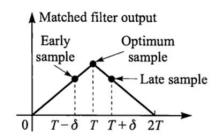
\includegraphics[width=4.00cm]{img_2.png}
\end{figure}
\subsection{Time equalization}
Représentation puis application de la fonction de transfert du canal. Pas nécessaire avec l'OFDM
\subsection{Frequency equalization}
Utile pour des modulations à large bande comme CDMA ou OFDM (variation de fréquence le long du canal). Dans le cas de l'OFDM on utilise l'interference inter-porteuse (ICI)
$$\hat{S}[k]=\frac{R[k]}{H[k]}$$
\subsubsection{Pilotes OFDM}
Continus ou intermittens mais prédéterminés. Modulés avec BPSK ou QPSK pour maximiser le SNR


\end{document}